\documentclass{article}
% [landscape]
\usepackage{amsmath, amsthm, amssymb, bm, color, framed, graphicx, hyperref, mathrsfs}
\usepackage{graphicx}%图片头文件
\usepackage{float} %指定图片位置
\usepackage{subfigure}%并排子图 共享标题 有子标题
\usepackage{caption}
\usepackage[margin=1in,letterpaper]{geometry} 

% code
\usepackage{listings} 
\usepackage{xcolor}
\lstset{
  language=Matlab,  %代码语言使用的是matlab
  frame=shadowbox, %把代码用带有阴影的框圈起来
  rulesepcolor=\color{red!20!green!20!blue!20},%代码块边框为淡青色
  keywordstyle=\color{blue!90}\bfseries, %代码关键字的颜色为蓝色,粗体
  commentstyle=\color{red!10!gray!70}\textit,    % 设置代码注释的颜色
  showstringspaces=false,%不显示代码字符串中间的空格标记
  numbers=left, % 显示行号
  numberstyle=\tiny,    % 行号字体
  stringstyle=\ttfamily, % 代码字符串的特殊格式
  breaklines=true, %对过长的代码自动换行
  extendedchars=false,  %解决代码跨页时,章节标题,页眉等汉字不显示的问题
%   escapebegin=\begin{CJK*},escapeend=\end{CJK*},      % 代码中出现中文必须加上,否则报错
  texcl=true}


\usepackage{ctex}
\usepackage{amsmath}
\usepackage{graphicx}
\usepackage{epstopdf}
\usepackage{tikz}
\usepackage{psfrag}
\usepackage{natbib}
\usepackage{hyperref}

\begin{document}

\renewcommand{\refname}{参考文献}
\renewcommand{\figurename}{图}
\renewcommand{\abstractname}{摘要}
% \def\due{2022 年 3 月 7 日周一 8:40}

\title{《磁流体力学的数值模拟方法》-- 第 2 次作业 \footnote{2022 春季《磁流体力学的数值模拟方法》}}


\author{蓝翔\footnote{Email: shsxjujishou@163.com
, 学号: SA21214038}
\and
康樨\footnote{Email: kx\_0045@mail.ustc.edu.cn, 学号: SA21007083}
\and
苏镇波\footnote{Email: zbsu@mail.ustc.edu.cn, 学号: SA21022002}
}

\date{%
\scriptsize%
%CAS Key Laboratory for Basic Plasma Physics, School of Earth and Space Sciences,
%\\
%University of Science and Technology of China, Hefei, Anhui 230026, China
中国科学技术大学核科学技术学院,合肥 230026\\
中国科学技术大学地球与空间科学学院, 合肥 230026\\
中国科学技术大学物理学院天文系, 合肥 230026
%
}

\maketitle

\begin{abstract}
在本次作业报告中,讨论一维单一变量双曲型方程 (行波方程和 Burgers 方程) 的有限差分数值解法 (迎风格式, Lax-Wodrff 格式, 前向欧拉格式以及蛙跳格式), 并结合理论分析讨论上述差分格式的特点.
\end{abstract}

\section{引言}
一维单变量函数的一阶双曲型偏微分方程表示了一个波动的传播发展过程, 在线性方程的情况下, 波的形状不随时间改变, 而在非线性方程的情况下, 一个连续有限振幅的波可能发展成有间断的解, 即激波, 或者从激波 (间断) 演化为连续的解 \citep{whitham2011}. 通过偏微分方程的数值计算格式, 可以分析数值解的物理特性和讨论格式的可靠性.
\section{方法及过程}
\subsection{行波方程}\label{xingbo}
考察方程:
\begin{equation}
    {\partial u\over\partial t} + {\partial u\over\partial x} = 0
\end{equation}

在初值条件:
\begin{equation}
\label{eq6}
u|_{t=0}=\left\{
\begin{aligned}
0.0 & , & x<-0.4, \\
1.0 - |x+0.3|/0.1 & , & -0.4 \leq x < -0.2, \\
0.0 & , & -0.2 \geq x < -0.1, \\
1.0 &, & -0.1 \geq < 0.0, \\
0.0 &, & x \leq 0.0
\end{aligned}
\right.
\end{equation}
下的数值解. 通过有限差分格式,如:

迎风格式
\begin{equation}
    u^{n+1}_{j} = u^n_j - {\Delta t\over\Delta x}(u^n_j - u^n_{j-1})
\end{equation}

Lax-Wendroff 格式:
\begin{equation}
    u^{n+1}_{j} = u^n_j - {a \Delta t\over 2\Delta x}(u^n_{j+1} - u^n_{j-1}) + {b \Delta t\over\Delta x^2}(u^n_{j+1} - 2u^n_j + u^n_{j-1})
\end{equation}

前向欧拉格式:
\begin{equation}
    u^{n+1}_{j} = u^n_j - {a \Delta t\over 2\Delta x}(u^n_{j+1} - u^n_{j-1})
\end{equation}


\subsection{Burgers 方程}
程序主要针对Burgers方程:
\begin{equation}
       {\partial u\over\partial t} + u{\partial u\over\partial x} = 0
\end{equation}
在初值为:
\begin{equation}
\label{eq6}
u|_{t=0}=\left\{
\begin{aligned}
1.8 & , & x<-0.8, \\
1.4 + 0.4cos[2\pi(x+0.8)] & , & -0.8 \leq x < 0.3, \\
1.0 & , & -0.3 \leq x < 0.0, \\
1.8 &, & x \qeq  0.0
\end{aligned}
\right.
\end{equation}
时的数值解. 采用了格式Upwind,Leapfrog,Lax进行数值计算。

对于较为特殊的Leapfrog格式,由于该格式联系了三个不同的时间层(n-1,n,n+1),需要对其使用启动格式以计算第2个时间层数值解(假设初始时刻解对应第1个时间层的解)。

其中,迎风格式Upwind以及Lax格式在第 \ref{xingbo} 节已叙述,这里仅表述 Leapfrog 格式:
\begin{equation}
    u^{n+1}_j = u^{n-1}_j - {a \Delta t\over \Delta x}(u^n_{j+1}-u^n_{j-1})+{2b\Delta t\over \Delta x^2}(u^n_{j+1}-u^{n+1}_j-u^{n-1}_j+u^n_{j-1}
\end{equation}

\section{实现,程序}
\subsection{行波方程}
\begin{figure}[H]
    \centering
    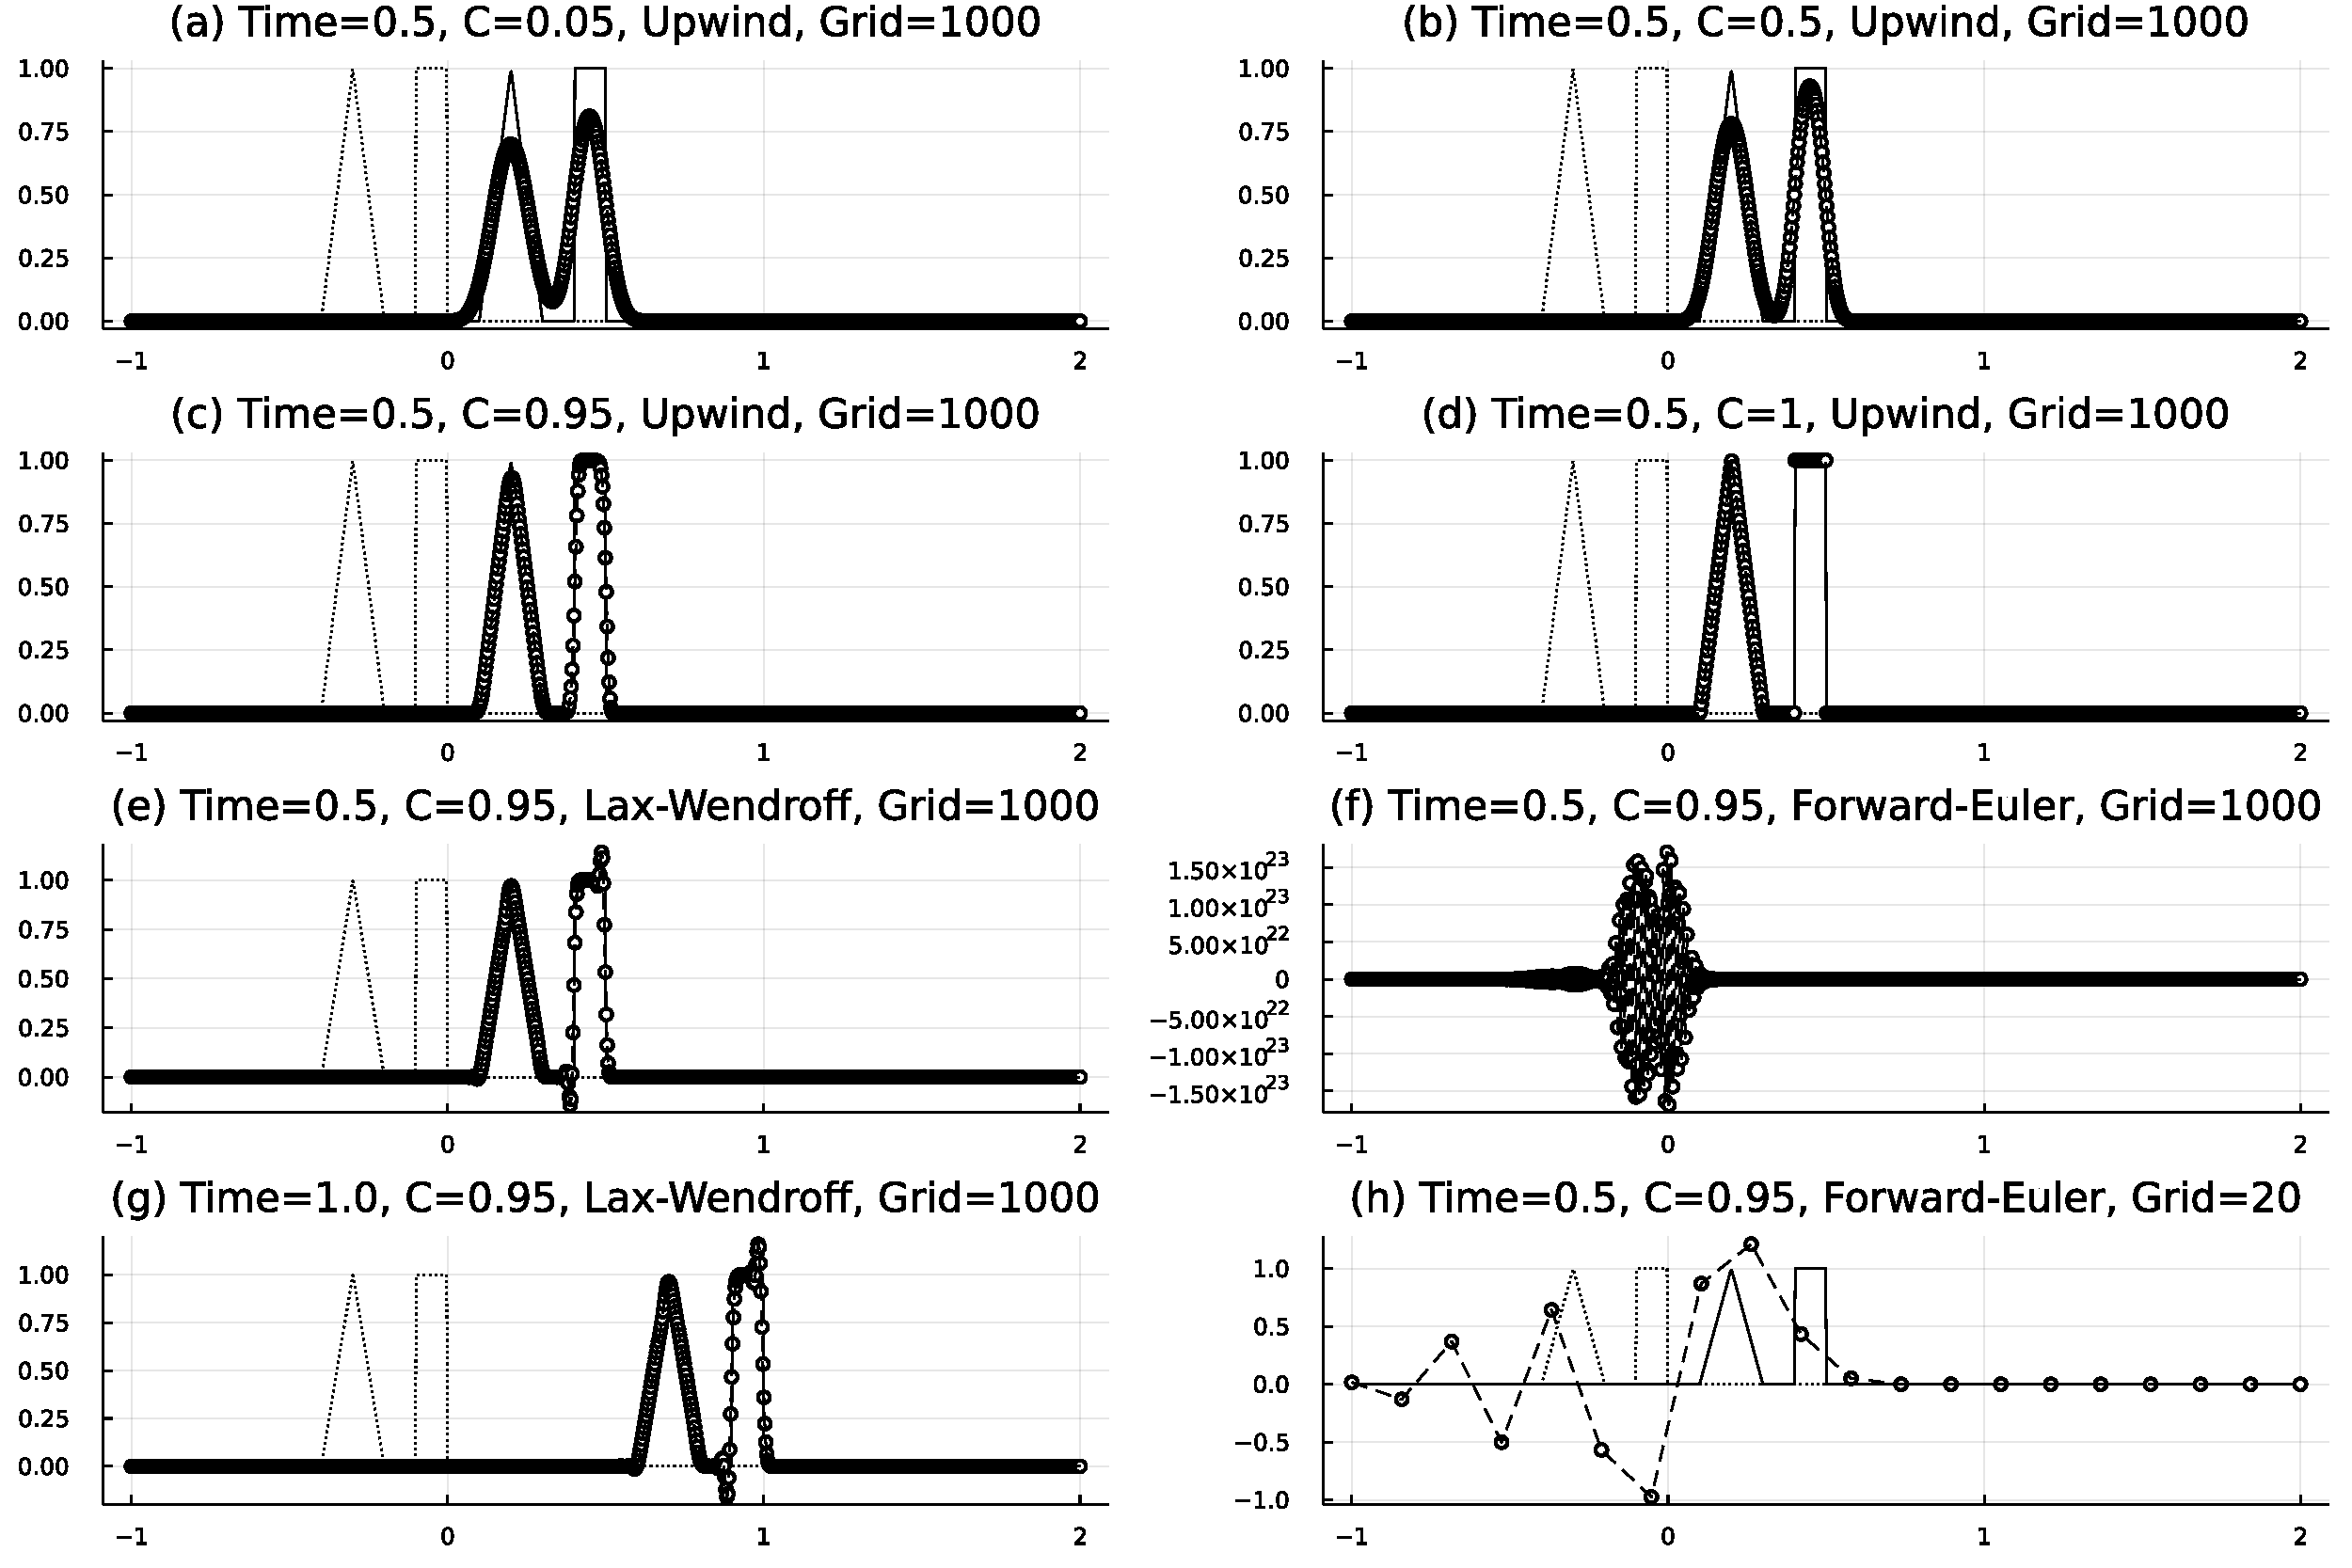
\includegraphics[width=1.0\textwidth]{hw2.pdf}
    \caption{方程 (1) 在 t = 0.5 (a-f, h) 和 t = 1.0 (g) 时刻的解. 除 (g) 外, 网格数均取1000. 其中虚线表示数值迎风格式的计算 结果, 线上的圆圈表示具体网格上的数据. 同一时刻的精确解用实线表示. 作为对照, 初始时刻的值以点线表示. (a) 迎风格式, C = 0.05, (b) 迎风格式, C = 0.50, (c) 迎风格式, C = 0.95, (d) 迎风格式, C = 1.0, 此时数值解与精确解完全相同, (e) Lax-Wendroff格式, C = 0.95, 注意其中出现的色散 (上冲和下冲), (f) Forward Euler格式, C = 0.95. (g) Lax-Wendroff格式, C = 0.95, t = 1.0, 同样出现色散. (h) Forward Euler格式, C = 0.95, 网格数取20. }
    \label{fig:1}
\end{figure}

\subsection{Burgers方程}

\begin{figure}[H]
    \centering
    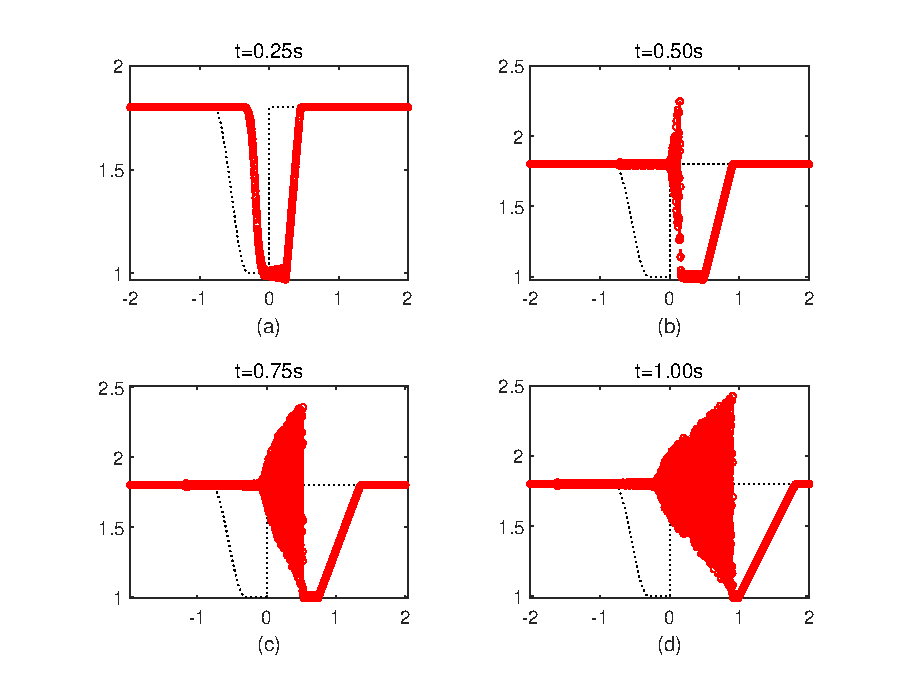
\includegraphics[width=0.5\textwidth]{Leapfrog.eps}
    \caption{(a)(b)(c)(d)四幅图分别是方程 (6)  Leapfrog格式下在时间t=0.25,0.50,0.75,1.00s时刻的数值解,此时C=0.5。其中红色点划线代表了数值解,黑色虚线代表了初始时刻解。}
    \label{fig:leapfrog2}
\end{figure}
\begin{figure}[H]
    \centering
    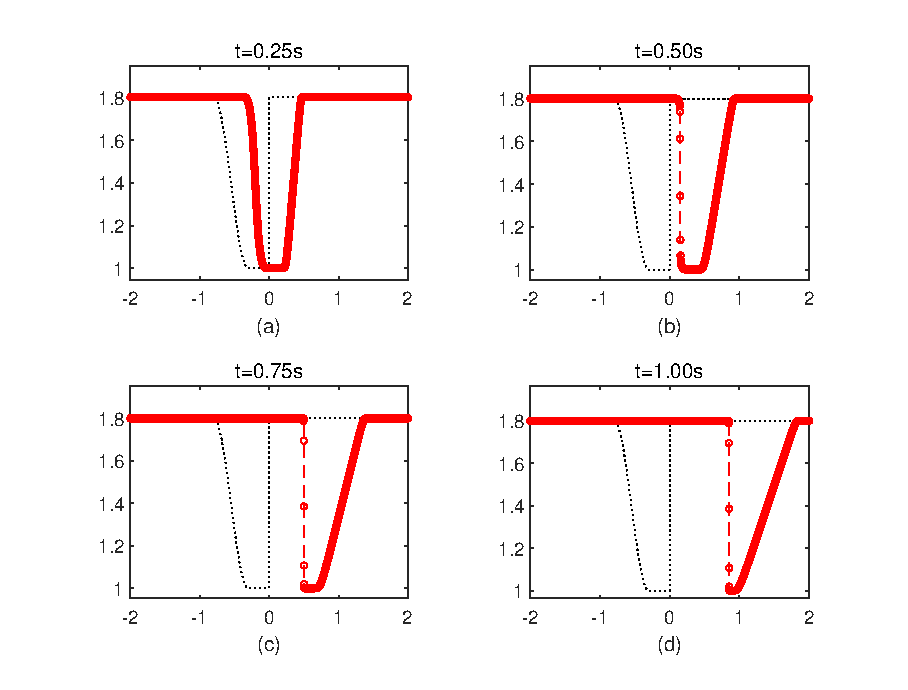
\includegraphics[width=0.5\textwidth]{Upwind.eps}
    \caption{(a)(b)(c)(d)四幅图分别是方程 (6) Upwind格式下在时间t=0.25,0.50,0.75,1.00s时刻的数值解,此时C=0.5。其中红色点划线代表了数值解,黑色虚线代表了初始时刻解。}
    \label{fig:upwind2}
\end{figure}
\begin{figure}[H]
    \centering
    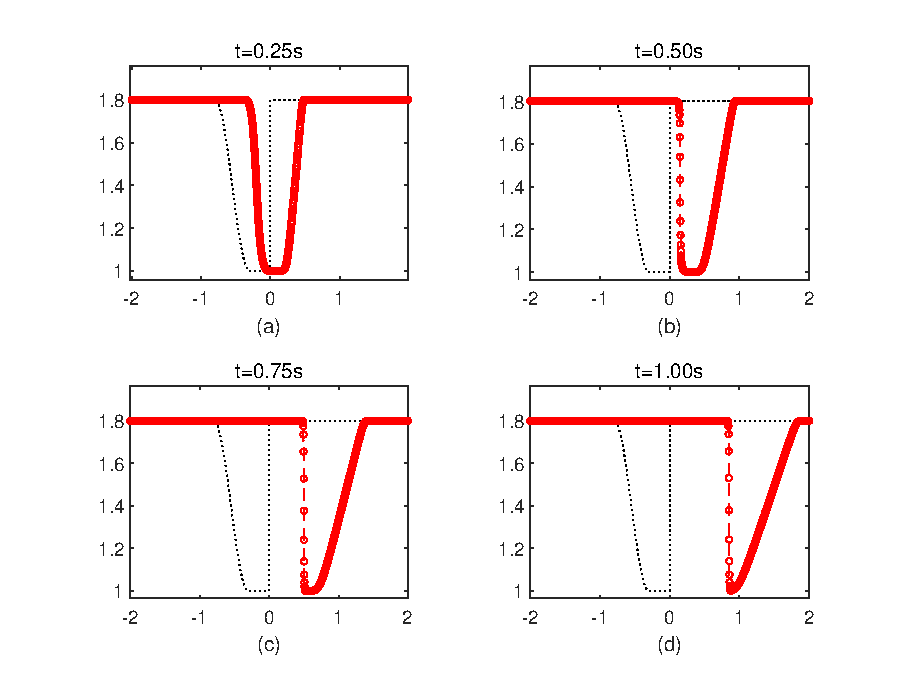
\includegraphics[width=0.5\textwidth]{Lax.eps}
    \caption{(a)(b)(c)(d)四幅图分别是方程 (6) Lax格式下在时间t=0.25,0.50,0.75,1.00s时刻的数值解,此时C=0.5。其中红色点划线代表了数值解,黑色虚线代表了初始时刻解。}
    \label{fig:lax2}
\end{figure}


\section{讨论,进一步工作}
\subsection{行波方程}

图 \ref{fig:1}中,不同 Courant 系数 ($C = \Delta t/\Delta x$), 在 t = 0.5 的计算结果,网格数取 1000 。 其中, 实线是精确解, 点线表示初态值, 虚线是数值计算结果, 而圆圈是具体网格 (单元) 上的数据。其中,图 \ref{fig:1} 的子图 (a) - (d) 分别对应在Upwind格式中 t=0.5 时,系数C分别取0.05, 0.5, 0.95, 1的情况,可以发现随着 Courant 系数的增加,数值解逐渐逼近精确解,在 $C=1$的时候,此时数值解与精确解完全相同;

图 \ref{fig:1} 的子图 (e) 中为 Lax-Wendroff 格式下 Courant 系数取 0.95 的情况, 网格数为1000,可以发现,在间断点处出现了明显的色散 (上冲和下冲);子图 (g) 中,t 取 1.0,发现和 t 取 0.5 的时候数值解的趋势大致相同,只是整个解向右移动。

图 \ref{fig:1} 的子图 (f) 中为空间向前差分的 Euler 格式在 Courant 系数取0.95、网格数取1000的情况,可以发现,空间向前差分的 Euler 格式相较于其他格式,出现了很明显的数值色散 (震荡) 。这是由于 Euler 格式中的缺点,随着网格数以及系数的增加,会引入不稳定的数值解。作为对比,可以在 (h) 中发现,当网格数取到 20 的时候,数值解的趋势大致和解析解一致,但是由于 Euler 格式的缺陷,有明显的色散存在。

通过对精确数值解波峰的移动,可以大致求得速度为0.4/s,间断区宽度大致为0.003。

\subsection{Burgers 方程}

由图 \ref{fig:leapfrog2} 可知,  Leapfrog格式相对Upwind格式最明显的特点是出现了震荡,即出现了数值色散。该震荡仅出现于数值解的波后位置且逐渐向波后远处扩展。以间段面附近震荡为例,该震荡振幅值接近0.8(最高点纵坐标接近2.6,最低点纵坐标接近1)。

可以看出在图 \ref{fig:upwind2} 中,随着时间增长,数值解的波形将会向x轴正向移动并且波形相对初始时刻会发生变形。可以认为在t=1.00s时刻精确解在横坐标约为0.85处有间断面,但由于数值耗散的缘故,图 \ref{fig:upwind2} (d) 中应存在间断面的地方被平滑产生间断宽度约为0.018;大致计算了t=0时x=0的点在不同时段的平均数值传播速度,发现0.25-0.50s内平均速度约为1.104/s,0.75-1.00s内平均速度约为1.392/s,可见该点平均数值传播速度随时间增长呈上升趋势;由于波前的移动速度要慢于波后的移动速度使得初始时刻的解逐渐变形产生了间断。

图 \ref{fig:lax2} 中Lax格式展现的性质同Upwind格式类似,不再赘述。

\section{分工说明}

苏镇波负责第一题,蓝翔完成了第二题,以及$\rm\LaTeX$的整理和排版.

\section{附件}

\begin{enumerate}
\item
MHD\_Group10.tex--本报告 \LaTeX 文件
\item
MHD\_Group10.pdf--本报告 PDF 输出文件
\item
code.txt--文中所用的 Julia 以及 Matlab 计算和图形绘制程序
\item
hw2.pdf--图~\ref{fig:1} 的 PDF 图形文件
\item
Leapfrog.eps--图~\ref{fig:leapfrog2} 的 EPS 图形文件
\item
Lax.eps--图~\ref{fig:lax2} 的 EPS 图形文件
\item
Upwind.eps--图~\ref{fig:upwind2} 的 EPS 图形文件
\item
References.bib -- 文献文件
\end{enumerate}

% 以下两行是中文文献国家标准的格式, 如果安装了这两个格式, 建议使用它们
% \bibliographystyle{gbt7714-author-year}
% \bibliographystyle{gbt7714-numerical}
%

%\bibliographystyle{unsrt}
\bibliographystyle{apalike}
\bibliography{References}

%\begin{thebibliography}{1}
%
%\bibitem{Diver2001}
%Declan~A. Diver.
%\newblock {\em A plasma formulary for physics, technology and astrophysics}.
%\newblock Wiley VCH, 1st edition, 2001.
%
%\bibitem{Jeffrey1964}
%A.~Jeffrey and T.~Taniuti.
%\newblock {\em Non-Linear Wave Propagation with Applications to Physics and
%  Magnetohydrodynamics}, volume~9 of {\em Mathematics in Science and
%  Engineering - A Series of Monographs and Textbooks}.
%\newblock Academic Press, New York / London, 1964.

%\end{thebibliography}

\end{document}
